\documentclass{standalone}% For the example only, any class will do

\usepackage{tikz}
\usetikzlibrary{positioning}% To get more advances positioning options
\usetikzlibrary{arrows,automata,positioning}
\usetikzlibrary{shapes.geometric}

\begin{document}
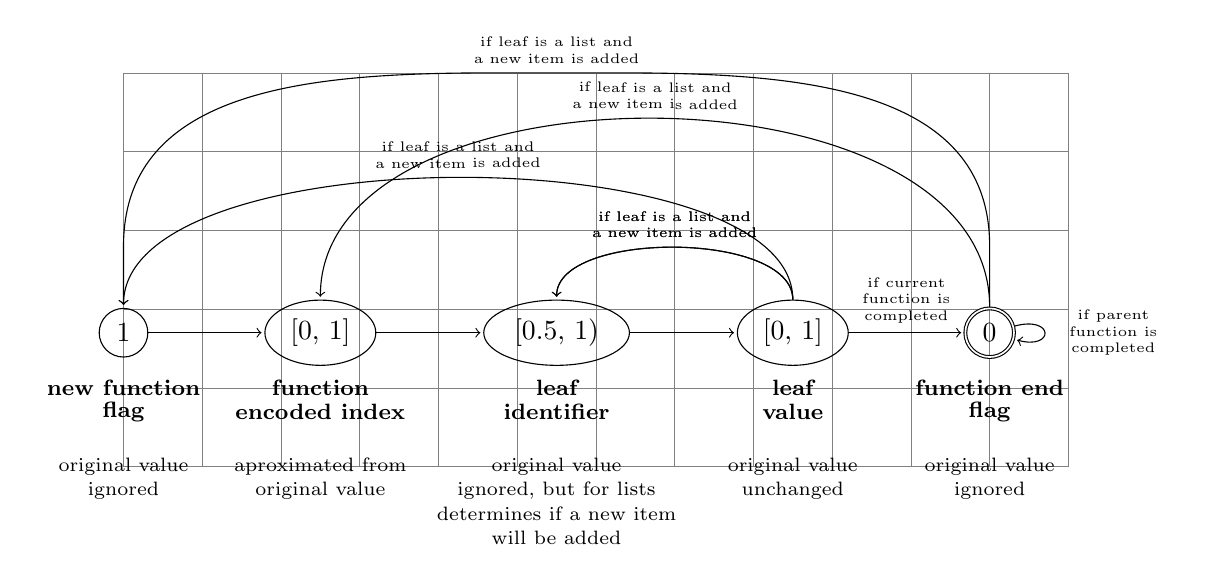
\begin{tikzpicture}[shorten >=1pt,node distance=2cm,auto]
\draw[help lines] (0,0) grid (12,5);

\node[circle,draw] (newF) at (0,1.7) {1};
\node[ellipse,draw] (funcEncIdx) at (2.5,1.7) {[0, 1]};
\node[ellipse,draw] (leafId) at (5.5,1.7) {[0.5, 1)};
\node[ellipse,draw] (leafValue) at (8.5,1.7) {[0, 1]};
\node[circle,draw,accepting] (funcEnd) at (11,1.7) {0};

\node[text width=2.2cm,text badly centered, font=\bfseries] at (0,1) {\footnotesize{new function}};
\node[text width=2.2cm,text badly centered, font=\bfseries] at (0,0.7) {\footnotesize{flag }};

\node[text width=2.2cm,text badly centered, font=\bfseries] at (2.5,1) {\footnotesize{function}};
\node[text width=2.2cm,text badly centered, font=\bfseries] at (2.5,0.7) {\footnotesize{encoded index}};

\node[text width=2.2cm,text badly centered, font=\bfseries] at (5.5,1) {\footnotesize{leaf}};
\node[text width=2.2cm,text badly centered, font=\bfseries] at (5.5,0.7) {\footnotesize{identifier}};

\node[text width=2.2cm,text badly centered, font=\bfseries] at (8.5,1) {\footnotesize{leaf}};
\node[text width=2.2cm,text badly centered, font=\bfseries] at (8.5,0.7) {\footnotesize{value}};

\node[text width=2.2cm,text badly centered, font=\bfseries] at (11,1) {\footnotesize{function end}};
\node[text width=2.2cm,text badly centered, font=\bfseries] at (11,0.7) {\footnotesize{flag }};


\node[text width=2.2cm,text badly centered] at (0,0) {\scriptsize{original value}};
\node[text width=2.2cm,text badly centered] at (0,-0.3) {\scriptsize{ignored }};

\node[text width=2.2cm,text badly centered] at (2.5,0) {\scriptsize{aproximated from}};
\node[text width=2.2cm,text badly centered] at (2.5,-0.3) {\scriptsize{original value }};

\node[text width=4.2cm,text badly centered] at (5.5,0) {\scriptsize{original value}};
\node[text width=4.2cm,text badly centered] at (5.5,-0.3) {\scriptsize{ignored, but for lists }};
\node[text width=4.2cm,text badly centered] at (5.5,-0.6) {\scriptsize{determines if a new item}};
\node[text width=4.2cm,text badly centered] at (5.5,-0.9) {\scriptsize{will be added}};

\node[text width=2.2cm,text badly centered] at (8.5,0) {\scriptsize{original value}};
\node[text width=2.2cm,text badly centered] at (8.5,-0.3) {\scriptsize{unchanged }};

\node[text width=2.2cm,text badly centered] at (11,0) {\scriptsize{original value}};
\node[text width=2.2cm,text badly centered] at (11,-0.3) {\scriptsize{ignored }};







      
     
\draw[->, font=\tiny, text width=2.1cm, text badly centered] (funcEnd) to [out=90,in=-90] (11,2.8)
      to [out=90,in=0] (5.5,5) node[above,sloped] {if leaf is a list and a new item is added} 
      to [out=180,in=90] (0,2.8) 
      to [out=270,in=90] (newF);

      
\path[->] (newF) edge node {} (funcEncIdx);     
\path[->] (funcEncIdx) edge node {} (leafId);
\path[->] (leafId) edge node {} (leafValue);
\path[->, font=\tiny, text width=1.5cm, text badly centered] (leafValue) edge node {if current function is completed} (funcEnd);

\path[->, font=\tiny, text width=1.5cm, text badly centered] (funcEnd) edge [loop right] node {if parent function is completed} (funcEnd);

\draw[->, font=\tiny, text width=2.1cm, text badly centered] (leafValue) .. controls +(up:1.3cm) and +(up:1.3cm) .. node[above,sloped] {if leaf is a list and a new item is added} (leafId);

\draw[->, font=\tiny, text width=2.1cm, text badly centered] (leafValue) .. controls +(up:1.3cm) and +(up:1.3cm) .. node[above,sloped] {if leaf is a list and a new item is added} (leafId);

\draw[->, font=\tiny, text width=2.1cm, text badly centered] (leafValue) .. controls +(up:2.5cm) and +(up:2.5cm) .. node[above,sloped] {if leaf is a list and a new item is added} (newF);

\draw[->, font=\tiny, text width=2.1cm, text badly centered] (funcEnd) .. controls +(up:3.5cm) and +(up:3.5cm) .. node[above,sloped] {if leaf is a list and a new item is added} (funcEncIdx);

% \draw[->, font=\tiny, text width=2.1cm, text badly centered] (funcEnd) .. controls +(up:4.5cm) and +(up:4.5cm) .. node[above,sloped] {if leaf is a list and a new item is added} (newF);


% (0,0) .. controls +(up:2cm) and +(left:3cm) .. (1,5)



%\node[state,initial] (q_newF) {$1$};
%
%
%\node[state] (q_funcEncIdx) [right of=q_newF] {$[0, 1]$};
%\node[state] (q_leafId) [right of=q_funcEncIdx] {$[0.5, 1)$};
%
%\node[state,accepting](q_3) [below right of=q_funcEncIdx] {$0$}; // end
%
%\path[->] (q_newF) edge node {0} (q_funcEncIdx);
% edge node [swap] {1} (q_2)
%(q_funcEncIdx) edge node {1} (q_3)
%edge [loop above] node {0} ()
%(q_2) edge node [swap] {0} (q_3)
% edge [loop below] node {1} ();
\end{tikzpicture}
\end{document}